\section{Initialisation}
\label{s:Initialisation}

\subsection{Stereo Initialisation}

\subsection{Monocular Initialisation}
The monocular initialisation is a key module in the Visual-Odometry pipeline.
It is ordered in the follwoing way:
\begin{enumerate}
	\item Find the 2D-2D correspondences between the the chosen first two images
	\item Apply the 8-point Algorithm to estimate the Fundamental matrix combined with running RANSAC.
	\item Check the validity of the estimated Fundamental matrix by either comparing the reprojection error or the distance to the epipolar line. 
	\item RANSAC return a set of inlier of the current 2D-2D correspondences.
	\item With the new set of inlier we can re-evaluate the final Essential Matrix $E$ estimate.
	\item The Essential Matrix $E$ can then be decomposed into two rotation and two translation hypotheses for the pose of the first camera frame. This gives in total a set of four camera motion possibilities.
	\item These hypotheses have to be disambiguated to choose the right camera rotation and translation.
\end{enumerate}

We have implemented two different approaches for finding the 2D-2D correspondences:

\begin{enumerate}
	\item Exercise implementation of Harris descriptor and detector.
	\item Implementation of the Kanade-Lucas Tracker (KLT).
\end{enumerate}

\begin{figure}
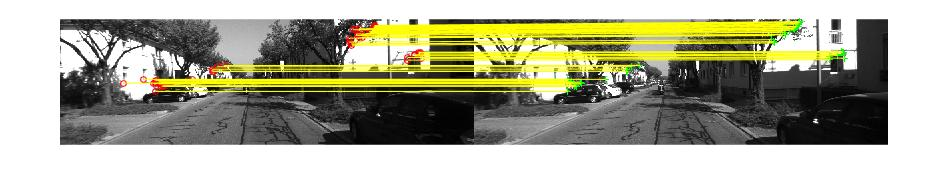
\includegraphics[width=0.98\textwidth]{files/KLT_2d2d.jpg}
\caption[\label{s:KLT_2d2d}]{2D-2D correspondences with KLT.}
\end{figure}

An examplary output of the 2D-2D module can be seen in Figure~\ref{s:KLT_2d2d}. The correspondences between two images are indicated.

Due to efficiency reasons we decided to use the epipolar line distance as a measure to validate the estimated Fundamental Matrices. In theory the reprojection error would have yielded better results (sacrificing efficiency); however, in our case the differences were neglectable.

\section{Continous Operation}
\label{s:ContOp}

\subsection{KLT}

\section{Bonus Features}
\label{s:BF}

\subsection{Plotting}


\subsection{Automatic Selection of Frames for Initialisation}

\subsection{Relocalisation}

\subsection{Full Bundle Adjustment}

\subsection{Calibrated Smartphone Camera and own Dataset}

\subsection{Quantitative Analysis}
\subsubsection{Keypoint Tracking via Block Matching versus KLT}
\subsection{Monocular Initialisation Harris Detector via Matlab versus Exercise Harris Detector}